% include a brief discussion about how the limitation of leaf instances affects the performance of the decision tree algorithm.

\documentclass[11pt,a4paper,twocolumn]{article}
% \usepackage{times} % times font
% \usepackage{mathptmx} % times font in maths
\usepackage[top=0.5in, bottom=0.6in, left=0.5in, right=0.5in]{geometry}
\usepackage{multirow} %in tables
\usepackage{caption} % in tables
\usepackage{lipsum}
\pagenumbering{gobble}
\newcommand{\HRule}{\rule{\linewidth}{0.5mm}}
\usepackage[pdftex]{graphicx}

% \usepackage{fullpage}
% \usepackage{amsmath}
% \usepackage{hyperref}
% \usepackage{graphicx}
% \usepackage{subfigure}
% \usepackage{indentfirst} % indent frst paragraph of section
% \usepackage[usenames,dvipsnames]{color}
% \newcommand{\ts}{\textsuperscript}

\begin{document}

\twocolumn[
\begin{@twocolumnfalse}
\begin{center}
	\begin{large}
	{\HRule \\[0.2cm]}
	\textsc{Assignment 2: Object Recognition--- Task 1}
	{\HRule \\[0.3cm]}
	\end{large}

{	\begin{minipage}{ 0.4\textwidth }
		\begin{flushleft}
			Kacper \textbf{Sokol} --- \texttt{ks1591}\\
			Maciej \textbf{Kumorek} --- \texttt{mk0934}
		\end{flushleft}
	\end{minipage}
	\begin{minipage}{ 0.4\textwidth }
		\begin{flushleft}
			{Image Processing \&\\ Computer Vision $|$ COMS30121}
		\end{flushleft}
	\end{minipage}
}

{\begin{small}
~\\[0.0000001cm]
\emph{Remark:} \textbf{FD}--- face(s) detected; \textbf{TP}--- true positive; \textbf{FP}--- false positive; \textbf{FN}--- false negative\\[0.0000001cm]
\end{small}}

\end{center}
\end{@twocolumnfalse}
]

\section*{Obama faces set}
\begin{itemize}
\item \texttt{obama0.jpg}--- 1 \textbf{FD}--- \textbf{TP}--- detection is pretty straight forward, whole face is visible--- model example of face for features detection.
\item \texttt{obama1.jpg}--- 0 \textbf{FD}--- \textbf{FN}--- the face is angled and features are not trained for rotated regions.
\item \texttt{obama2.jpg}--- 1 \textbf{FD}--- \textbf{TP}--- eyes, nose, ears or hair are clearly visible in image so features are easily matched.
\item \texttt{obama3.jpg}--- 0 \textbf{FD}--- \textbf{FN}--- the light reflection covered half of face what stopped classifier from matching basic face features.
\item \texttt{obama4.jpg}--- 2 \textbf{FD}--- \textbf{TP}, \textbf{FP}--- enough part of face was visible to collect needed features to recognize it (sunglasses enforce dark eyes region matching). The other detection is incorrect. The gradual change of blue color matched with facial features is visible(\textit{Figure:\ref{img:false-positive}}) possibly due to \textit{jpg} compression.
\item \texttt{obama5.jpg}--- 0 \textbf{FD}--- \textbf{FN}--- half of the face is covered what prevents classifier from matching features such as eyes(dark region) or nose(bridge).
\item \texttt{obama6.jpg}--- 4 \textbf{FD}--- \textbf{TP}, 3 \textbf{FP}--- the face is detected but 3 other objects are misclassified. Shading of the hand could resemble human face. Dark square mis-recognized is similar to \texttt{obama4} case. Mouth are detected as face possibly due to: black circular shadow formed in the corner of the lips-- face, upper lip-- eyes and tooth-- nose.
\item \texttt{obama7.jpg}--- 0 \textbf{FD}--- \textbf{FN}--- the face is undetected because of the side view-- no symmetrical features visible: eyes with nose in-between.
\item \texttt{obama8.jpg}--- 0 \textbf{FD}--- \textbf{FN}--- the face is not found because of different proportions due to horizontal distortion, what leads to features(eyes, nose) not being matched.
\item \texttt{obama9.jpg}--- 0 \textbf{FD}--- \textbf{FN}--- shaded eyes together with left facial profile result in undetected face.
\item \texttt{obama10.jpg}--- 1 \textbf{FD}--- \textbf{TP}--- all characteristic features of face are visible leading to correct detection.
\item \texttt{obama11.jpg}--- 2 \textbf{FD}--- \textbf{TP}, \textbf{FP}--- even though face is distorted all features are visible and give correct classification. Second detection is incorrect possibly because of similar reasons as in \texttt{obama6}.
\end{itemize}

\begin{figure}[htbp]
\centering
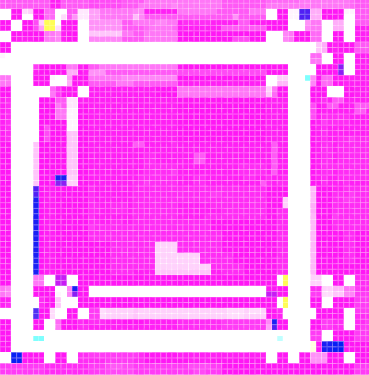
\includegraphics[width=0.1\textwidth]{false-positive.png}
\caption{False positive in \texttt{obama4.jpg}.\label{img:false-positive}\\[0.0000000000000000000000000000001cm]}
\end{figure}

\section*{Team faces set}
\begin{itemize}
\item \texttt{team0.jpg}--- 1 \textbf{FD}--- \textbf{TP}--- the frontal view of face results in correct recognition.
\item \texttt{team1.jpg}--- 2 \textbf{FD}--- \textbf{TP}, \textbf{FP}--- visible face is correctly recognized as it is frontal picture. The second detection is incorrect possibly due to glasses being recognized as mouth and hair pattern being similar to eyes.
\item \texttt{team2.jpg}--- 1 \textbf{FD}--- \textbf{TP}--- frontal face photo provides all basic features.
\item \texttt{team3.jpg}--- 0 \textbf{FD}--- \textbf{FP}--- hair covering face(eyes, nose) prevent classifier from recognizing it.
\item \texttt{team4.jpg}--- 1 \textbf{FD}--- \textbf{TP}--- even though mouth is covered eyes and nose matched with corresponding features are enough to find a face.
\item \texttt{team5.jpg}--- 2 \textbf{FD}--- \textbf{TP}, \textbf{FP}--- the face is found despite small bottom region covered. Second detection is wrong possibly due to similar reasons as in \texttt{team1}.
\end{itemize}

\section*{Conclusions}
Used features and classifier behave very good with near frontal face photos with non or very small regions covered. Other views are hardly ever recognized with sometimes noise or random objects being misclassified.

\end{document}
